\section{Signal Model}%
\label{sec:model}

\begin{figure}[t]
  \centerline{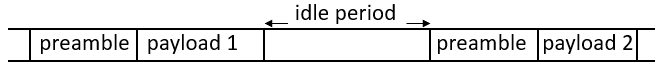
\includegraphics[width=3.4in]{data_structure.png}}
  \caption{Structure of signal stream at the receiver}
  \label{fig:data_structure}
  \end{figure}

In our model, the transmitted bursts are separated by an unkown length of idle period and assumed to
include a reference signal (preamble) that is known to the receiver;
see Figure~\ref{fig:data_structure}. 
%Often such a reference sequence is prepended to the payload and is referred to as a preamble.
%The structure of signal stream at the receiver is shown in Figure~\ref{fig:data_structure}. 
The problem addressed in this paper is to accurately estimate the
start time of the preamble and to estimate carrier phase and frequency
offset from the preamble. 
The payload portion of the burst is not further considered. 
% Moreover, to make our algorithm applicable for signal transmission in very high speed,
% the complexity of algorithm is also crucial.

%We now give the signal model for this paper.
The received signal is modeled at base band.
In~\cite{Morelli_Mengali_98} and~\cite{Ramakrishnan_10}, 
the authors obtain a simplifed signal model from the matched filter
outputs;
however, this assumes that the symbol time is perfectly known.
Also, the matched filter frontend is not optimal in the presence of
frequency offset.
In contrast, our model assumes that the received signal is
oversampled: we collect $M$ samples per symbol period $T$, i.e., the
sample period is $T_s=\frac{T}{M}$. 
The received samples $r_n$ are given by the model
\begin{equation}
    \begin{aligned}
      \label{eq:model}
      r_p = s_{p-\bar{p}}Ae^{j\phi}e^{j2\pi\delta p}+w_{p},
    \end{aligned}
  \end{equation}
where the reference sequence (preamble) $s_n$ is constructed from
$L_0$ known reference symbols $c_i$ using pulse shaping $g(t)$
\begin{equation}
  \label{eq:l_ref_sig_discrete}
  s_n=\sum_{i=0}^{L_0-1} c_i g(nT_s-iT) \quad \text{for}~n=0,\ldots,N-1.
  % \begin{dcases}
  %   \sum_{i=0}^{L_0-1} c_i g(nT_s-iT) & \text{for}~n=0,\ldots,N-1, \\
  %   0 & \text{otherwise}.
  % \end{dcases}
\end{equation}
The preamble consists of $N=M L_0$ samples.  
  
In~\eqref{eq:model}, $\bar{p}$ denotes the start
position\footnote{This implies that delay is quantized to
  $\bar{p}T_s$. We assume that the signal is oversampled sufficiently
  that the quantization error is negligible.} of the received preamble.
% Note, because of the uncertainty of sampling, often the sampler may not sample exactly at the start time of the preamble, which causes
% the integer delay $\bar{p}$ with a fractional delay in the range of $[-\frac{T_s}{2},\frac{T_s}{2})$, where $T_s$ is the sample period as in~\eqref{eq:l_ref_sig_discrete}.
% In this paper, the sampling rate is assumed to be high enough relative to the symbol rate, so that the influence of fractional delay can be ignored.
$A$, $\phi$, $\delta$ are the amplitude, carrier phase and normalized
(by $T_s$)
frequency offset.
%that we want to estimate.
$w_p$ is complex AWGN.\@
Moreover, we will denote by $E_s/N_0$ the ratio of signal energy to noise power spectral density (SNR).
To simplify analysis, we assume a constant and normalized envelope of the samples in the 
preamble, i.e., $A^2|s_n|^2\approx A^2=E_s/M$ for $n=[0,N-1]$.

In this paper, two time axes are relevant. A global time axis, denoted
by $p$, measures the position of samples in the entire received
stream. A local time axis, denoted by $n$, refers to sample indices
within the preamble (see~\eqref{eq:model}
and~\eqref{eq:l_ref_sig_discrete}).
The local time-axis $n$ is also used in each step of the sequential
detector where a window of $N$ samples is processed.

% Finally, note that in~\eqref{eq:l_ref_sig_discrete}, when the discrete time index $n$ of $s_n$ is greater than $N-1$,
% or equivalently, $n>p+N-1$ in~\eqref{eq:model}, it means the received samples $r_n$ at those $n$ are in the payload;
% We assume the data of payload is zero for simplicity (normally it isn't) because it does not affect the time synchronization of the preamble and carrier synchronization from the preamble.


% The rest of paper includes two main sections. The first section (Section 3 and 4) focus on 
% analyzing the signal acquisition chain, which includes the sequential detection process and
% carrier synchronization of the preamble. The above block diagram is shown in Figure 2.
% The simulation section 5 then illustrates the performance of proposed algorithm
% in the first section. The second section (section 6) moves attention on implementing the algorithm on software-defined radio (SDR).
% Some steps (equations) in the first section are computed more efficiently to achieve the best throughput.